\documentclass[12pt]{article}
\author{Lawrence Liu}
\usepackage{subcaption}
\usepackage{graphicx}
\usepackage{amsmath}
\usepackage{pdfpages}
\newcommand{\Laplace}{\mathscr{L}}
\setlength{\parskip}{\baselineskip}%
\setlength{\parindent}{0pt}%
\usepackage{xcolor}
\usepackage{listings}
\definecolor{backcolour}{rgb}{0.95,0.95,0.92}
\usepackage{amssymb}
\lstdefinestyle{mystyle}{
    backgroundcolor=\color{backcolour}}
\lstset{style=mystyle}

\title{ECE 113 HW 1}
\begin{document}
\maketitle
\section*{Problem 1}
\subsection*{(a)}
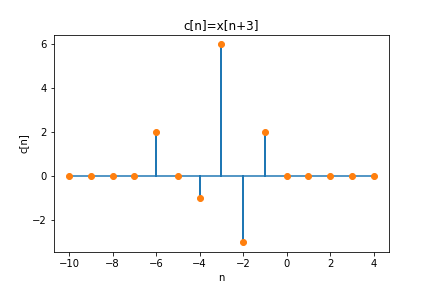
\includegraphics[scale=0.5]{c.png}
\subsection*{(b)}
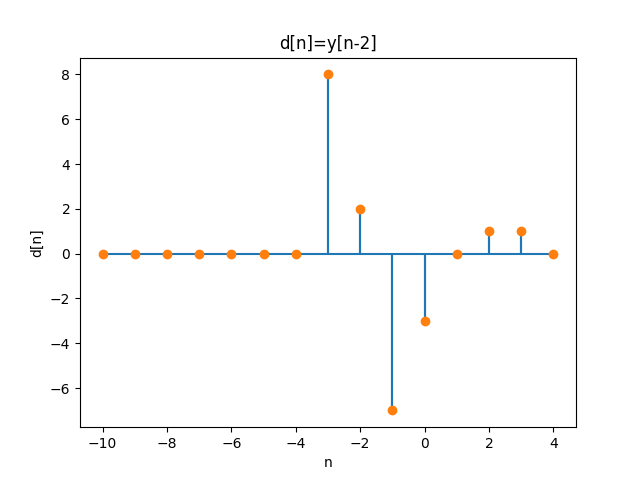
\includegraphics[scale=0.5]{d.png}
\subsection*{(c)}
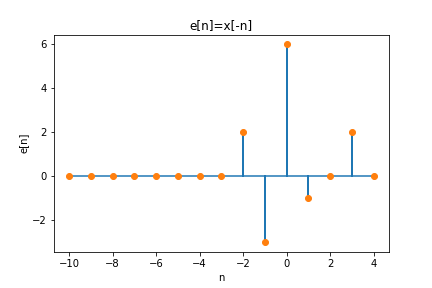
\includegraphics[scale=0.5]{e.png}
\subsection*{(d)}
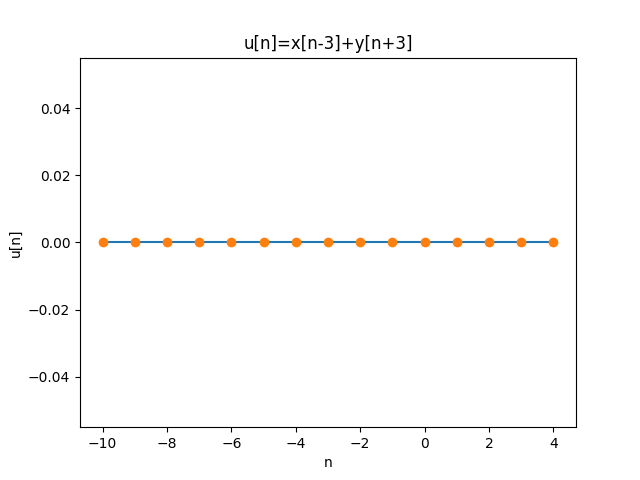
\includegraphics[scale=0.5]{u.png}
\subsection*{(e)}
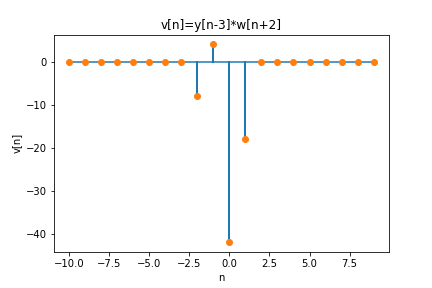
\includegraphics[scale=0.5]{v.png}
\subsection*{(f)}
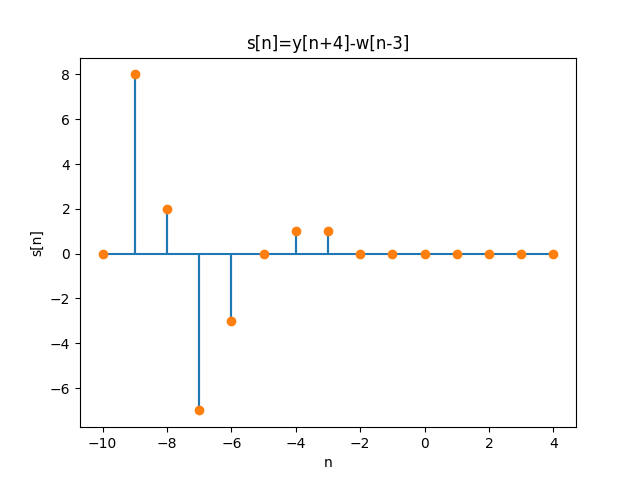
\includegraphics[scale=0.5]{s.png}
\subsection*{(g)}
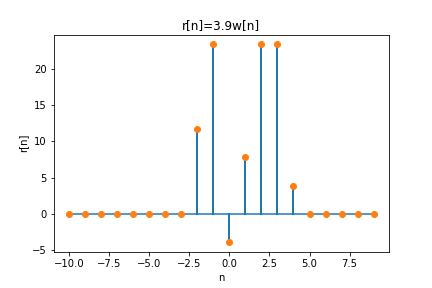
\includegraphics[scale=0.5]{r.png}
\section*{Problem 2}
\subsection*{(a)}
$$\boxed{20}$$
\subsection*{(b)}
$$\boxed{25}$$
\subsection*{(c)}
$$\boxed{40}$$
\subsection*{(d)}
$$\boxed{80}$$
\subsection*{(e)}
$$\boxed{20}$$
\subsection*{(f)}
$$\boxed{8}$$
\section*{Problem 3}
\subsection*{(a)}
Since $e^{j\theta} = \cos(\theta) + j\sin(\theta)$, we have
that the fundamental period of $\hat{x}_a[n]$ is $\boxed{8}$
\subsection*{(b)}
We have that $F_0=0.3$, therefore we have that the period of the sequence
is $\frac{k}{0.3}$. The minimum $k$ such that this evaluates to a
positive integer is $k=3$. Therefore, the fundamental period of
the sequence is $\boxed{10}$.




\end{document}
